\documentclass{standalone}
\usepackage{tikz}
\begin{document}
% Created by tikzDevice version 0.7.0 on 2014-12-04 16:52:38
% !TEX encoding = UTF-8 Unicode
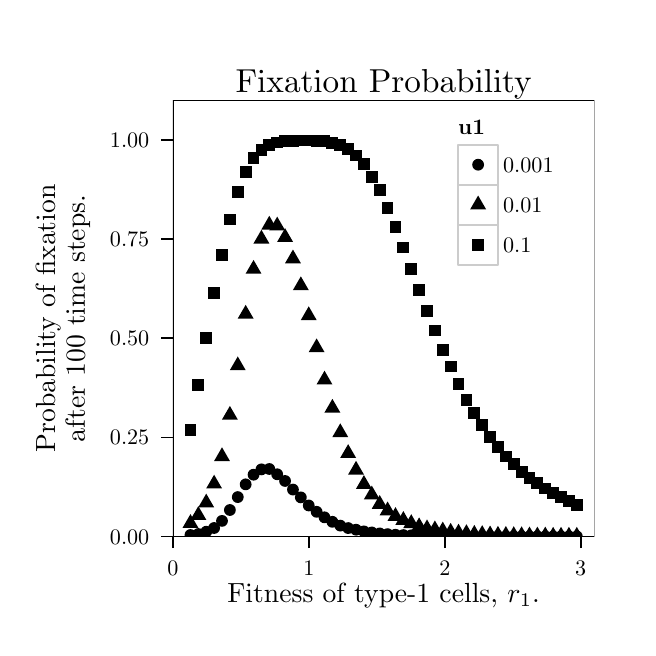
\begin{tikzpicture}[x=1pt,y=1pt]
\definecolor[named]{fillColor}{rgb}{1.00,1.00,1.00}
\path[use as bounding box,fill=fillColor,fill opacity=0.00] (0,0) rectangle (216.81,216.81);
\begin{scope}
\path[clip] (  0.00,  0.00) rectangle (216.81,216.81);
\definecolor[named]{drawColor}{rgb}{1.00,1.00,1.00}
\definecolor[named]{fillColor}{rgb}{1.00,1.00,1.00}

\path[draw=drawColor,line width= 0.6pt,line join=round,line cap=round,fill=fillColor] (  0.00,  0.00) rectangle (216.81,216.81);
\end{scope}
\begin{scope}
\path[clip] ( 52.49, 32.98) rectangle (204.77,190.48);
\definecolor[named]{fillColor}{rgb}{1.00,1.00,1.00}

\path[fill=fillColor] ( 52.49, 32.98) rectangle (204.77,190.48);
\definecolor[named]{fillColor}{rgb}{0.00,0.00,0.00}

\path[fill=fillColor] ( 56.69, 69.42) --
	( 60.96, 69.42) --
	( 60.96, 73.69) --
	( 56.69, 73.69) --
	cycle;

\path[fill=fillColor] ( 59.54, 85.49) --
	( 63.81, 85.49) --
	( 63.81, 89.76) --
	( 59.54, 89.76) --
	cycle;

\path[fill=fillColor] ( 62.39,102.65) --
	( 66.66,102.65) --
	( 66.66,106.91) --
	( 62.39,106.91) --
	cycle;

\path[fill=fillColor] ( 65.24,118.91) --
	( 69.50,118.91) --
	( 69.50,123.17) --
	( 65.24,123.17) --
	cycle;

\path[fill=fillColor] ( 68.09,132.56) --
	( 72.35,132.56) --
	( 72.35,136.83) --
	( 68.09,136.83) --
	cycle;

\path[fill=fillColor] ( 70.93,145.36) --
	( 75.20,145.36) --
	( 75.20,149.62) --
	( 70.93,149.62) --
	cycle;

\path[fill=fillColor] ( 73.78,155.22) --
	( 78.05,155.22) --
	( 78.05,159.49) --
	( 73.78,159.49) --
	cycle;

\path[fill=fillColor] ( 76.63,162.38) --
	( 80.90,162.38) --
	( 80.90,166.65) --
	( 76.63,166.65) --
	cycle;

\path[fill=fillColor] ( 79.48,167.46) --
	( 83.75,167.46) --
	( 83.75,171.73) --
	( 79.48,171.73) --
	cycle;

\path[fill=fillColor] ( 82.33,170.37) --
	( 86.60,170.37) --
	( 86.60,174.64) --
	( 82.33,174.64) --
	cycle;

\path[fill=fillColor] ( 85.18,172.26) --
	( 89.45,172.26) --
	( 89.45,176.52) --
	( 85.18,176.52) --
	cycle;

\path[fill=fillColor] ( 88.03,173.16) --
	( 92.30,173.16) --
	( 92.30,177.42) --
	( 88.03,177.42) --
	cycle;

\path[fill=fillColor] ( 90.88,173.60) --
	( 95.15,173.60) --
	( 95.15,177.87) --
	( 90.88,177.87) --
	cycle;

\path[fill=fillColor] ( 93.73,173.79) --
	( 98.00,173.79) --
	( 98.00,178.06) --
	( 93.73,178.06) --
	cycle;

\path[fill=fillColor] ( 96.58,173.89) --
	(100.84,173.89) --
	(100.84,178.16) --
	( 96.58,178.16) --
	cycle;

\path[fill=fillColor] ( 99.43,173.89) --
	(103.69,173.89) --
	(103.69,178.16) --
	( 99.43,178.16) --
	cycle;

\path[fill=fillColor] (102.27,173.82) --
	(106.54,173.82) --
	(106.54,178.09) --
	(102.27,178.09) --
	cycle;

\path[fill=fillColor] (105.12,173.64) --
	(109.39,173.64) --
	(109.39,177.91) --
	(105.12,177.91) --
	cycle;

\path[fill=fillColor] (107.97,173.08) --
	(112.24,173.08) --
	(112.24,177.34) --
	(107.97,177.34) --
	cycle;

\path[fill=fillColor] (110.82,172.31) --
	(115.09,172.31) --
	(115.09,176.58) --
	(110.82,176.58) --
	cycle;

\path[fill=fillColor] (113.67,170.89) --
	(117.94,170.89) --
	(117.94,175.16) --
	(113.67,175.16) --
	cycle;

\path[fill=fillColor] (116.52,168.49) --
	(120.79,168.49) --
	(120.79,172.76) --
	(116.52,172.76) --
	cycle;

\path[fill=fillColor] (119.37,165.31) --
	(123.64,165.31) --
	(123.64,169.58) --
	(119.37,169.58) --
	cycle;

\path[fill=fillColor] (122.22,160.76) --
	(126.49,160.76) --
	(126.49,165.02) --
	(122.22,165.02) --
	cycle;

\path[fill=fillColor] (125.07,155.92) --
	(129.34,155.92) --
	(129.34,160.19) --
	(125.07,160.19) --
	cycle;

\path[fill=fillColor] (127.92,149.62) --
	(132.18,149.62) --
	(132.18,153.89) --
	(127.92,153.89) --
	cycle;

\path[fill=fillColor] (130.77,142.56) --
	(135.03,142.56) --
	(135.03,146.83) --
	(130.77,146.83) --
	cycle;

\path[fill=fillColor] (133.61,135.26) --
	(137.88,135.26) --
	(137.88,139.53) --
	(133.61,139.53) --
	cycle;

\path[fill=fillColor] (136.46,127.54) --
	(140.73,127.54) --
	(140.73,131.81) --
	(136.46,131.81) --
	cycle;

\path[fill=fillColor] (139.31,119.82) --
	(143.58,119.82) --
	(143.58,124.08) --
	(139.31,124.08) --
	cycle;

\path[fill=fillColor] (142.16,112.36) --
	(146.43,112.36) --
	(146.43,116.62) --
	(142.16,116.62) --
	cycle;

\path[fill=fillColor] (145.01,105.24) --
	(149.28,105.24) --
	(149.28,109.51) --
	(145.01,109.51) --
	cycle;

\path[fill=fillColor] (147.86, 98.20) --
	(152.13, 98.20) --
	(152.13,102.47) --
	(147.86,102.47) --
	cycle;

\path[fill=fillColor] (150.71, 92.28) --
	(154.98, 92.28) --
	(154.98, 96.54) --
	(150.71, 96.54) --
	cycle;

\path[fill=fillColor] (153.56, 85.82) --
	(157.83, 85.82) --
	(157.83, 90.09) --
	(153.56, 90.09) --
	cycle;

\path[fill=fillColor] (156.41, 80.26) --
	(160.68, 80.26) --
	(160.68, 84.53) --
	(156.41, 84.53) --
	cycle;

\path[fill=fillColor] (159.26, 75.58) --
	(163.52, 75.58) --
	(163.52, 79.84) --
	(159.26, 79.84) --
	cycle;

\path[fill=fillColor] (162.11, 71.05) --
	(166.37, 71.05) --
	(166.37, 75.32) --
	(162.11, 75.32) --
	cycle;

\path[fill=fillColor] (164.95, 66.81) --
	(169.22, 66.81) --
	(169.22, 71.08) --
	(164.95, 71.08) --
	cycle;

\path[fill=fillColor] (167.80, 63.19) --
	(172.07, 63.19) --
	(172.07, 67.45) --
	(167.80, 67.45) --
	cycle;

\path[fill=fillColor] (170.65, 59.70) --
	(174.92, 59.70) --
	(174.92, 63.96) --
	(170.65, 63.96) --
	cycle;

\path[fill=fillColor] (173.50, 56.89) --
	(177.77, 56.89) --
	(177.77, 61.16) --
	(173.50, 61.16) --
	cycle;

\path[fill=fillColor] (176.35, 54.25) --
	(180.62, 54.25) --
	(180.62, 58.52) --
	(176.35, 58.52) --
	cycle;

\path[fill=fillColor] (179.20, 51.89) --
	(183.47, 51.89) --
	(183.47, 56.16) --
	(179.20, 56.16) --
	cycle;

\path[fill=fillColor] (182.05, 50.05) --
	(186.32, 50.05) --
	(186.32, 54.32) --
	(182.05, 54.32) --
	cycle;

\path[fill=fillColor] (184.90, 48.16) --
	(189.17, 48.16) --
	(189.17, 52.42) --
	(184.90, 52.42) --
	cycle;

\path[fill=fillColor] (187.75, 46.40) --
	(192.01, 46.40) --
	(192.01, 50.66) --
	(187.75, 50.66) --
	cycle;

\path[fill=fillColor] (190.60, 44.94) --
	(194.86, 44.94) --
	(194.86, 49.21) --
	(190.60, 49.21) --
	cycle;

\path[fill=fillColor] (193.45, 43.57) --
	(197.71, 43.57) --
	(197.71, 47.83) --
	(193.45, 47.83) --
	cycle;

\path[fill=fillColor] (196.29, 42.32) --
	(200.56, 42.32) --
	(200.56, 46.59) --
	(196.29, 46.59) --
	cycle;

\path[fill=fillColor] ( 58.82, 41.03) --
	( 61.70, 36.05) --
	( 55.95, 36.05) --
	cycle;

\path[fill=fillColor] ( 61.67, 43.93) --
	( 64.55, 38.96) --
	( 58.80, 38.96) --
	cycle;

\path[fill=fillColor] ( 64.52, 48.44) --
	( 67.40, 43.46) --
	( 61.65, 43.46) --
	cycle;

\path[fill=fillColor] ( 67.37, 55.28) --
	( 70.24, 50.30) --
	( 64.50, 50.30) --
	cycle;

\path[fill=fillColor] ( 70.22, 65.18) --
	( 73.09, 60.20) --
	( 67.35, 60.20) --
	cycle;

\path[fill=fillColor] ( 73.07, 80.13) --
	( 75.94, 75.16) --
	( 70.19, 75.16) --
	cycle;

\path[fill=fillColor] ( 75.92, 98.01) --
	( 78.79, 93.03) --
	( 73.04, 93.03) --
	cycle;

\path[fill=fillColor] ( 78.77,116.66) --
	( 81.64,111.68) --
	( 75.89,111.68) --
	cycle;

\path[fill=fillColor] ( 81.62,132.88) --
	( 84.49,127.90) --
	( 78.74,127.90) --
	cycle;

\path[fill=fillColor] ( 84.47,143.79) --
	( 87.34,138.81) --
	( 81.59,138.81) --
	cycle;

\path[fill=fillColor] ( 87.31,148.83) --
	( 90.19,143.85) --
	( 84.44,143.85) --
	cycle;

\path[fill=fillColor] ( 90.16,148.53) --
	( 93.04,143.55) --
	( 87.29,143.55) --
	cycle;

\path[fill=fillColor] ( 93.01,144.38) --
	( 95.89,139.40) --
	( 90.14,139.40) --
	cycle;

\path[fill=fillColor] ( 95.86,136.64) --
	( 98.74,131.66) --
	( 92.99,131.66) --
	cycle;

\path[fill=fillColor] ( 98.71,126.95) --
	(101.58,121.97) --
	( 95.84,121.97) --
	cycle;

\path[fill=fillColor] (101.56,116.12) --
	(104.43,111.14) --
	( 98.69,111.14) --
	cycle;

\path[fill=fillColor] (104.41,104.52) --
	(107.28, 99.54) --
	(101.53, 99.54) --
	cycle;

\path[fill=fillColor] (107.26, 92.85) --
	(110.13, 87.88) --
	(104.38, 87.88) --
	cycle;

\path[fill=fillColor] (110.11, 82.68) --
	(112.98, 77.71) --
	(107.23, 77.71) --
	cycle;

\path[fill=fillColor] (112.96, 73.84) --
	(115.83, 68.86) --
	(110.08, 68.86) --
	cycle;

\path[fill=fillColor] (115.81, 66.32) --
	(118.68, 61.35) --
	(112.93, 61.35) --
	cycle;

\path[fill=fillColor] (118.65, 60.29) --
	(121.53, 55.31) --
	(115.78, 55.31) --
	cycle;

\path[fill=fillColor] (121.50, 55.14) --
	(124.38, 50.16) --
	(118.63, 50.16) --
	cycle;

\path[fill=fillColor] (124.35, 51.33) --
	(127.23, 46.35) --
	(121.48, 46.35) --
	cycle;

\path[fill=fillColor] (127.20, 47.94) --
	(130.08, 42.96) --
	(124.33, 42.96) --
	cycle;

\path[fill=fillColor] (130.05, 45.60) --
	(132.92, 40.62) --
	(127.18, 40.62) --
	cycle;

\path[fill=fillColor] (132.90, 43.57) --
	(135.77, 38.60) --
	(130.03, 38.60) --
	cycle;

\path[fill=fillColor] (135.75, 42.14) --
	(138.62, 37.16) --
	(132.87, 37.16) --
	cycle;

\path[fill=fillColor] (138.60, 40.99) --
	(141.47, 36.01) --
	(135.72, 36.01) --
	cycle;

\path[fill=fillColor] (141.45, 39.85) --
	(144.32, 34.87) --
	(138.57, 34.87) --
	cycle;

\path[fill=fillColor] (144.30, 39.10) --
	(147.17, 34.13) --
	(141.42, 34.13) --
	cycle;

\path[fill=fillColor] (147.14, 38.74) --
	(150.02, 33.77) --
	(144.27, 33.77) --
	cycle;

\path[fill=fillColor] (149.99, 38.32) --
	(152.87, 33.34) --
	(147.12, 33.34) --
	cycle;

\path[fill=fillColor] (152.84, 37.87) --
	(155.72, 32.89) --
	(149.97, 32.89) --
	cycle;

\path[fill=fillColor] (155.69, 37.56) --
	(158.57, 32.59) --
	(152.82, 32.59) --
	cycle;

\path[fill=fillColor] (158.54, 37.38) --
	(161.42, 32.40) --
	(155.67, 32.40) --
	cycle;

\path[fill=fillColor] (161.39, 37.13) --
	(164.26, 32.15) --
	(158.52, 32.15) --
	cycle;

\path[fill=fillColor] (164.24, 37.04) --
	(167.11, 32.06) --
	(161.37, 32.06) --
	cycle;

\path[fill=fillColor] (167.09, 36.91) --
	(169.96, 31.93) --
	(164.21, 31.93) --
	cycle;

\path[fill=fillColor] (169.94, 36.79) --
	(172.81, 31.81) --
	(167.06, 31.81) --
	cycle;

\path[fill=fillColor] (172.79, 36.74) --
	(175.66, 31.76) --
	(169.91, 31.76) --
	cycle;

\path[fill=fillColor] (175.64, 36.66) --
	(178.51, 31.68) --
	(172.76, 31.68) --
	cycle;

\path[fill=fillColor] (178.48, 36.63) --
	(181.36, 31.65) --
	(175.61, 31.65) --
	cycle;

\path[fill=fillColor] (181.33, 36.55) --
	(184.21, 31.58) --
	(178.46, 31.58) --
	cycle;

\path[fill=fillColor] (184.18, 36.51) --
	(187.06, 31.53) --
	(181.31, 31.53) --
	cycle;

\path[fill=fillColor] (187.03, 36.52) --
	(189.91, 31.54) --
	(184.16, 31.54) --
	cycle;

\path[fill=fillColor] (189.88, 36.43) --
	(192.75, 31.45) --
	(187.01, 31.45) --
	cycle;

\path[fill=fillColor] (192.73, 36.45) --
	(195.60, 31.47) --
	(189.86, 31.47) --
	cycle;

\path[fill=fillColor] (195.58, 36.45) --
	(198.45, 31.47) --
	(192.71, 31.47) --
	cycle;

\path[fill=fillColor] (198.43, 36.42) --
	(201.30, 31.44) --
	(195.55, 31.44) --
	cycle;

\path[fill=fillColor] ( 58.82, 33.49) circle (  2.13);

\path[fill=fillColor] ( 61.67, 33.84) circle (  2.13);

\path[fill=fillColor] ( 64.52, 34.67) circle (  2.13);

\path[fill=fillColor] ( 67.37, 36.02) circle (  2.13);

\path[fill=fillColor] ( 70.22, 38.58) circle (  2.13);

\path[fill=fillColor] ( 73.07, 42.52) circle (  2.13);

\path[fill=fillColor] ( 75.92, 47.19) circle (  2.13);

\path[fill=fillColor] ( 78.77, 51.79) circle (  2.13);

\path[fill=fillColor] ( 81.62, 55.27) circle (  2.13);

\path[fill=fillColor] ( 84.47, 57.20) circle (  2.13);

\path[fill=fillColor] ( 87.31, 57.34) circle (  2.13);

\path[fill=fillColor] ( 90.16, 55.43) circle (  2.13);

\path[fill=fillColor] ( 93.01, 53.01) circle (  2.13);

\path[fill=fillColor] ( 95.86, 49.90) circle (  2.13);

\path[fill=fillColor] ( 98.71, 47.08) circle (  2.13);

\path[fill=fillColor] (101.56, 44.16) circle (  2.13);

\path[fill=fillColor] (104.41, 41.87) circle (  2.13);

\path[fill=fillColor] (107.26, 39.87) circle (  2.13);

\path[fill=fillColor] (110.11, 38.25) circle (  2.13);

\path[fill=fillColor] (112.96, 36.88) circle (  2.13);

\path[fill=fillColor] (115.81, 35.99) circle (  2.13);

\path[fill=fillColor] (118.65, 35.40) circle (  2.13);

\path[fill=fillColor] (121.50, 34.79) circle (  2.13);

\path[fill=fillColor] (124.35, 34.41) circle (  2.13);

\path[fill=fillColor] (127.20, 34.06) circle (  2.13);

\path[fill=fillColor] (130.05, 33.80) circle (  2.13);

\path[fill=fillColor] (132.90, 33.58) circle (  2.13);

\path[fill=fillColor] (135.75, 33.46) circle (  2.13);

\path[fill=fillColor] (138.60, 33.37) circle (  2.13);

\path[fill=fillColor] (141.45, 33.29) circle (  2.13);

\path[fill=fillColor] (144.30, 33.20) circle (  2.13);

\path[fill=fillColor] (147.14, 33.18) circle (  2.13);

\path[fill=fillColor] (149.99, 33.17) circle (  2.13);

\path[fill=fillColor] (152.84, 33.11) circle (  2.13);

\path[fill=fillColor] (155.69, 33.09) circle (  2.13);

\path[fill=fillColor] (158.54, 33.05) circle (  2.13);

\path[fill=fillColor] (161.39, 33.02) circle (  2.13);

\path[fill=fillColor] (164.24, 33.03) circle (  2.13);

\path[fill=fillColor] (167.09, 33.03) circle (  2.13);

\path[fill=fillColor] (169.94, 33.01) circle (  2.13);

\path[fill=fillColor] (172.79, 33.01) circle (  2.13);

\path[fill=fillColor] (175.64, 33.00) circle (  2.13);

\path[fill=fillColor] (178.48, 32.99) circle (  2.13);

\path[fill=fillColor] (181.33, 32.99) circle (  2.13);

\path[fill=fillColor] (184.18, 33.00) circle (  2.13);

\path[fill=fillColor] (187.03, 32.99) circle (  2.13);

\path[fill=fillColor] (189.88, 32.99) circle (  2.13);

\path[fill=fillColor] (192.73, 32.98) circle (  2.13);

\path[fill=fillColor] (195.58, 32.99) circle (  2.13);

\path[fill=fillColor] (198.43, 32.99) circle (  2.13);
\definecolor[named]{drawColor}{rgb}{0.00,0.00,0.00}

\path[draw=drawColor,line width= 0.6pt,line join=round,line cap=round] ( 52.49, 32.98) rectangle (204.77,190.48);
\end{scope}
\begin{scope}
\path[clip] (  0.00,  0.00) rectangle (216.81,216.81);
\definecolor[named]{drawColor}{rgb}{0.00,0.00,0.00}

\node[text=drawColor,anchor=base east,inner sep=0pt, outer sep=0pt, scale=  0.80] at ( 43.95, 30.22) {0.00};

\node[text=drawColor,anchor=base east,inner sep=0pt, outer sep=0pt, scale=  0.80] at ( 43.95, 66.02) {0.25};

\node[text=drawColor,anchor=base east,inner sep=0pt, outer sep=0pt, scale=  0.80] at ( 43.95,101.81) {0.50};

\node[text=drawColor,anchor=base east,inner sep=0pt, outer sep=0pt, scale=  0.80] at ( 43.95,137.61) {0.75};

\node[text=drawColor,anchor=base east,inner sep=0pt, outer sep=0pt, scale=  0.80] at ( 43.95,173.40) {1.00};
\end{scope}
\begin{scope}
\path[clip] (  0.00,  0.00) rectangle (216.81,216.81);
\definecolor[named]{drawColor}{rgb}{0.00,0.00,0.00}

\path[draw=drawColor,line width= 0.6pt,line join=round] ( 48.22, 32.98) --
	( 52.49, 32.98);

\path[draw=drawColor,line width= 0.6pt,line join=round] ( 48.22, 68.77) --
	( 52.49, 68.77);

\path[draw=drawColor,line width= 0.6pt,line join=round] ( 48.22,104.57) --
	( 52.49,104.57);

\path[draw=drawColor,line width= 0.6pt,line join=round] ( 48.22,140.36) --
	( 52.49,140.36);

\path[draw=drawColor,line width= 0.6pt,line join=round] ( 48.22,176.16) --
	( 52.49,176.16);
\end{scope}
\begin{scope}
\path[clip] (  0.00,  0.00) rectangle (216.81,216.81);
\definecolor[named]{drawColor}{rgb}{0.00,0.00,0.00}

\path[draw=drawColor,line width= 0.6pt,line join=round] ( 52.49, 28.71) --
	( 52.49, 32.98);

\path[draw=drawColor,line width= 0.6pt,line join=round] (101.61, 28.71) --
	(101.61, 32.98);

\path[draw=drawColor,line width= 0.6pt,line join=round] (150.73, 28.71) --
	(150.73, 32.98);

\path[draw=drawColor,line width= 0.6pt,line join=round] (199.85, 28.71) --
	(199.85, 32.98);
\end{scope}
\begin{scope}
\path[clip] (  0.00,  0.00) rectangle (216.81,216.81);
\definecolor[named]{drawColor}{rgb}{0.00,0.00,0.00}

\node[text=drawColor,anchor=base,inner sep=0pt, outer sep=0pt, scale=  0.80] at ( 52.49, 18.93) {0};

\node[text=drawColor,anchor=base,inner sep=0pt, outer sep=0pt, scale=  0.80] at (101.61, 18.93) {1};

\node[text=drawColor,anchor=base,inner sep=0pt, outer sep=0pt, scale=  0.80] at (150.73, 18.93) {2};

\node[text=drawColor,anchor=base,inner sep=0pt, outer sep=0pt, scale=  0.80] at (199.85, 18.93) {3};
\end{scope}
\begin{scope}
\path[clip] (  0.00,  0.00) rectangle (216.81,216.81);
\definecolor[named]{drawColor}{rgb}{0.00,0.00,0.00}

\node[text=drawColor,anchor=base,inner sep=0pt, outer sep=0pt, scale=  1.00] at (128.63,  9.03) {Fitness of type-1 cells, $r_1$.};
\end{scope}
\begin{scope}
\path[clip] (  0.00,  0.00) rectangle (216.81,216.81);
\definecolor[named]{drawColor}{rgb}{0.00,0.00,0.00}

\node[text=drawColor,rotate= 90.00,anchor=base,inner sep=0pt, outer sep=0pt, scale=  1.00] at (  9.90,111.73) {Probability of fixation };

\node[text=drawColor,rotate= 90.00,anchor=base,inner sep=0pt, outer sep=0pt, scale=  1.00] at ( 20.70,111.73) {  after 100 time steps.};
\end{scope}
\begin{scope}
\path[clip] (  0.00,  0.00) rectangle (216.81,216.81);
\definecolor[named]{fillColor}{rgb}{1.00,1.00,1.00}

\path[fill=fillColor] (151.28,126.89) rectangle (194.29,187.92);
\end{scope}
\begin{scope}
\path[clip] (  0.00,  0.00) rectangle (216.81,216.81);
\definecolor[named]{drawColor}{rgb}{0.00,0.00,0.00}

\node[text=drawColor,anchor=base west,inner sep=0pt, outer sep=0pt, scale=  0.80] at (155.55,178.13) {\bfseries u1};
\end{scope}
\begin{scope}
\path[clip] (  0.00,  0.00) rectangle (216.81,216.81);
\definecolor[named]{drawColor}{rgb}{0.80,0.80,0.80}
\definecolor[named]{fillColor}{rgb}{1.00,1.00,1.00}

\path[draw=drawColor,line width= 0.6pt,line join=round,line cap=round,fill=fillColor] (155.55,160.06) rectangle (170.00,174.52);
\end{scope}
\begin{scope}
\path[clip] (  0.00,  0.00) rectangle (216.81,216.81);
\definecolor[named]{fillColor}{rgb}{0.00,0.00,0.00}

\path[fill=fillColor] (162.77,167.29) circle (  2.13);
\end{scope}
\begin{scope}
\path[clip] (  0.00,  0.00) rectangle (216.81,216.81);
\definecolor[named]{drawColor}{rgb}{0.80,0.80,0.80}
\definecolor[named]{fillColor}{rgb}{1.00,1.00,1.00}

\path[draw=drawColor,line width= 0.6pt,line join=round,line cap=round,fill=fillColor] (155.55,145.61) rectangle (170.00,160.06);
\end{scope}
\begin{scope}
\path[clip] (  0.00,  0.00) rectangle (216.81,216.81);
\definecolor[named]{fillColor}{rgb}{0.00,0.00,0.00}

\path[fill=fillColor] (162.77,156.15) --
	(165.65,151.18) --
	(159.90,151.18) --
	cycle;
\end{scope}
\begin{scope}
\path[clip] (  0.00,  0.00) rectangle (216.81,216.81);
\definecolor[named]{drawColor}{rgb}{0.80,0.80,0.80}
\definecolor[named]{fillColor}{rgb}{1.00,1.00,1.00}

\path[draw=drawColor,line width= 0.6pt,line join=round,line cap=round,fill=fillColor] (155.55,131.15) rectangle (170.00,145.61);
\end{scope}
\begin{scope}
\path[clip] (  0.00,  0.00) rectangle (216.81,216.81);
\definecolor[named]{fillColor}{rgb}{0.00,0.00,0.00}

\path[fill=fillColor] (160.64,136.25) --
	(164.91,136.25) --
	(164.91,140.52) --
	(160.64,140.52) --
	cycle;
\end{scope}
\begin{scope}
\path[clip] (  0.00,  0.00) rectangle (216.81,216.81);
\definecolor[named]{drawColor}{rgb}{0.00,0.00,0.00}

\node[text=drawColor,anchor=base west,inner sep=0pt, outer sep=0pt, scale=  0.80] at (171.81,164.53) {0.001};
\end{scope}
\begin{scope}
\path[clip] (  0.00,  0.00) rectangle (216.81,216.81);
\definecolor[named]{drawColor}{rgb}{0.00,0.00,0.00}

\node[text=drawColor,anchor=base west,inner sep=0pt, outer sep=0pt, scale=  0.80] at (171.81,150.08) {0.01};
\end{scope}
\begin{scope}
\path[clip] (  0.00,  0.00) rectangle (216.81,216.81);
\definecolor[named]{drawColor}{rgb}{0.00,0.00,0.00}

\node[text=drawColor,anchor=base west,inner sep=0pt, outer sep=0pt, scale=  0.80] at (171.81,135.63) {0.1};
\end{scope}
\begin{scope}
\path[clip] (  0.00,  0.00) rectangle (216.81,216.81);
\definecolor[named]{drawColor}{rgb}{0.00,0.00,0.00}

\node[text=drawColor,anchor=base,inner sep=0pt, outer sep=0pt, scale=  1.20] at (128.63,193.49) {Fixation Probability};
\end{scope}
\end{tikzpicture}
\end{document}
